\documentclass[11pt, letterpaper]{article}

\makeatletter
\makeatother
\usepackage[hidelinks]{hyperref}
\usepackage{comment}
\usepackage{enumitem}
\usepackage{fullpage}
\usepackage[english]{babel}
\usepackage[utf8x]{inputenc}
\usepackage{amsmath}
\usepackage{amssymb}
\usepackage{graphicx}
\usepackage[colorinlistoftodos]{todonotes}
\usepackage[linesnumbered]{algorithm2e}
\usepackage{tabularx}
\usepackage{url}
\usepackage{hyperref}
\hypersetup{colorlinks=true}
\usepackage[margin=0.5in]{geometry}    % For reducing margin
\usepackage[english]{babel}
\usepackage{mathtools}
\usepackage{booktabs}
\usepackage{physics}
\usepackage{float}
\usepackage{xcolor}
\newcommand{\wx}[1]{\textcolor{magenta}{\bf\small [#1 --WX]}}


\begin{document}
\title{CS 4650: Natural Language Processing \\ Spring 2022 \\ Problem Set 2}
\author{Instructor: Dr. Wei Xu \\ TAs: Chao Jiang, Chase Perry, Rucha Sathe \\Piazza: \url{https://piazza.com/gatech/spring2022/cs4650a}}
\date{Due: Tuesday, Mar 1, 11:59pm ET}
\maketitle

\section{Word Embeddings}

The \textsc{Word2Vec} algorithm revolutionized the field of NLP by providing a high-quality, but cheaply computable means for producing continuous vector representations of words learned from a large, unlabelled corpus. Here, we will investigate the objectives used in the \textsc{Word2Vec} algorithm. This question may require you to refer to Chapters 14.5, 14.6 of the Eisenstein readings. \\

Here is a sentence for which the algorithm will make a prediction for the missing word. The word embedding for each word in the context has been given.

\begin{table}[h!]
    \centering
    \begin{tabular}{|ccc|}
    \toprule
    \textbf{Index Position} & \textbf{Word} & \textbf{Embedding} \\
    \midrule
    0 & apples & $[-2,10,-18]$ \\
    1 & and & $[8,-2,4]$ \\
    2 & ? & ? \\
    3 & are & $[0,-2,4]$\\
    4 & closely & $[-2,-2,2]$\\
    5 & related & $[0,4,2]$\\
    6 & to & $[0,-6,10]$\\
    7 & each & $[4,-2,10]$\\
    8 & other & $[0,12,-16]$\\
    
    \bottomrule
    \end{tabular}
    \caption{Word Embeddings for the Input Sentence.}
\end{table}

\begin{enumerate}
    \item (\textbf{2 pt}) Compute the Continuous Bag-of-Words (CBOW) vector representation of the missing word for a context window $h$ of size 2. Show your work.
    
    \item (\textbf{5 pts}) We've subset the vocabulary down to the words in Table \ref{tab:vocab}. Fill in the scores of each word being the missing word in Table \ref{tab:vocab}. Use the base-2 exponent and round to 2 decimal places.\\
    Hint: use dot products for this, not traditional vector-space similarity.
    
\begin{table}[H]
    \centering
    \begin{tabular}{|c|c|c|c|}
    \toprule
    \textbf{Word} & \textbf{Embedding} & \textbf{Unnormalized Score} & \textbf{Normalized Score (P(Word))}\\
    \midrule
    oranges & $[-6,4,-4]$ & & \\
    \hline
    pineapples & $[-8,1,-6]$ & & \\
    \hline
    pies & $[0,-4, -3]$ & & \\
    \hline
    doctors & $[3,0, -1]$ & & \\
    \hline
    witches & $[2,1,0]$ & & \\
    \bottomrule
    \end{tabular}
    \label{tab:vocab}
    \caption{A subset of the vocabulary of the CBOW model.}
\end{table}
    
    \item (\textbf{1 pt}) Which word would be predicted by the CBOW algorithm to be the missing word?

\end{enumerate}

\section{Hidden Markov Models and the Viterbi Algorithm}
    We have a toy language with 2 words - “cool” and “shade”. We want to tag the parts of speech in a test corpus in this toy language. There are only 2 parts of speech — NN (noun) and VB (verb) in this language. We have a corpus of text in which we the following distribution of the 2 words:
    
    \begin{table}[h!]
    \centering
    \small
    \begin{tabular}{|l | c | c |}
    \hline & NN & VB\\
    \hline
    cool & 4 & 8 \\
    shade & 6 & 2\\
    \hline
    \end{tabular}
    \end{table}
    Assume that we have an HMM model with the following transition probabilities (* is a special start of the sentence symbol).
    
    \begin{figure}[H]
    \centering
    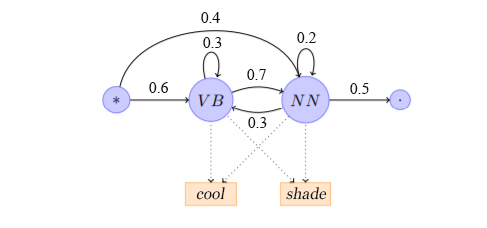
\includegraphics{images/HMM.jpg}
    \caption{HMM model for POS tagging in our toy language.}
    \end{figure}

\begin{enumerate}
\item (\textbf{2 pts}) Compute the emission probabilities for each word given each POS tag.\\

\item (\textbf{3 pts}) Draw the Viterbi trellis for the sequence “cool shade.”. Highlight the most likely sequence. \href{https://web.stanford.edu/~jurafsky/slp3/A.pdf#page=8}{\color{blue}{Here}} is an  example of Viterbi trellis.

\end{enumerate}

\section{Named Entity Recognition} 

Consider a sentence that contains three named entities (organization name, person name, location name) and the predictions from four automatic name entity recognition systems. What is the entity-level Precision, Recall, and F1-score of each system's performance? Here, we do not consider giving any credits to partial matches. \\\\

    \begin{tabular}{|c|c|c|c|c|c|c|c|c|c|}
    \hline
    Sentence   & \text{\tt Microsoft} & \text{\tt founder} & \text{\tt Bill} & \text{\tt Gates} & \text{\tt grew} & \text{\tt up} & \text{\tt in} & \text{\tt Seattle} \\
         \hline
    Gold Labels & B-ORG & O & B-PER & I-PER & O & O & O & B-LOC \\
            \hline
    System \#1      & B-ORG & O & B-PER & O & O & O & O & B-LOC \\
                \hline
    System \#2      & B-ORG & O & B-PER & I-PER & O & O & O & B-LOC \\        
                \hline
    System \#3      & B-ORG & B-PER & O & O & O & O & O & B-LOC \\
                \hline
    System \#4      & B-ORG & O & O & B-PER & O & O & O & B-LOC \\
    \hline            
    \end{tabular}

    \vspace{.5in}
For each system compute:

\begin{enumerate}[label=(\alph*)]
    \item (\textbf{2 pts}) Precision
    \item (\textbf{2 pts}) Recall
    \item (\textbf{2 pts}) F-1 score
\end{enumerate}

\noindent You may refer to Chapter 8.3 of the Eisenstein readings to learn more about the concept and notations used in NER.

\end{document}